\documentclass[11pt,a4paper]{article}

\usepackage[T1]{fontenc}
\usepackage[utf8]{inputenc}
\usepackage[spanish]{babel}
\usepackage[margin=2.5cm]{geometry}
\usepackage{graphicx}
\usepackage{amsmath}
\usepackage{booktabs}
\usepackage[font=small,labelfont=bf,skip=6pt]{caption}
\usepackage{placeins}
\usepackage[hidelinks]{hyperref}
\addto\captionsspanish{\renewcommand{\tablename}{Tabla}}

% Permitir que las figuras compartan página con el texto.
\renewcommand{\topfraction}{0.9}
\renewcommand{\bottomfraction}{0.8}
\renewcommand{\textfraction}{0.08}
\renewcommand{\floatpagefraction}{0.85}
\setlength{\textfloatsep}{14pt plus 2pt minus 2pt}
\setlength{\intextsep}{12pt plus 2pt minus 2pt}
\clubpenalty=10000
\widowpenalty=10000

% Carpetas donde buscar imágenes, relativas a report/.
\graphicspath{{figures/}{../data/images/}{../data/contours/}}

\title{Reporte de segmentación con GrabCut}
\author{Franco Castro Chaves\\C01886 \and Emily Chacón Araya\\C02047}
\date{}

\begin{document}

\maketitle

\begin{abstract}
% !TeX root = main.tex
Se estudia una implementación de segmentación interactiva basada en
GrabCut para delimitar schwannoma vestibular en cortes de resonancia
magnética. El conjunto de trabajo comprende 30 imágenes PNG asociadas a
la colección Vestibular-Schwannoma-SEG. El procedimiento inicializa las
etiquetas mediante un rectángulo, modela las intensidades de fondo y primer
plano con cinco gaussianas por clase y alterna la actualización de estos
modelos con cortes mínimos en un grafo de ocho vecinos. La evaluación
presentada corresponde al caso \texttt{VS-SEG-001} y utiliza una máscara
binaria extraída de su anotación roja. Tras cinco iteraciones, se
obtuvieron 47 falsos positivos y 84 falsos negativos, con un error
cuadrático medio de $0{,}000500$ sobre la imagen completa y de
$0{,}026422$ dentro del rectángulo. Las discrepancias se redujeron un
$92{,}25$~\% respecto de una predicción de todo fondo. Las etiquetas
permanecieron sin cambios desde la tercera iteración hasta la quinta,
aunque los modelos de intensidad continuaron actualizándose. El
análisis ilustra el comportamiento del procedimiento en el corte seleccionado.

\end{abstract}

\tableofcontents
\newpage

% !TeX root = main.tex
\section{Introducción}
\label{sec:introduccion}

La segmentación de imágenes asigna etiquetas a los píxeles para delimitar
regiones de interés~\cite{szeliski2011}. En una imagen de resonancia magnética, la delimitación
de una lesión requiere distinguirla de los tejidos circundantes a partir
de su apariencia y de su organización espacial. Cuando distintas regiones
presentan intensidades semejantes, una clasificación basada únicamente en
la intensidad puede producir ambigüedades. Incorporar relaciones entre
píxeles vecinos permite favorecer regiones coherentes, mientras que una
selección interactiva restringe la búsqueda a la zona de interés~\cite{boykov2001}.

GrabCut combina modelos de apariencia de fondo y primer plano con una
penalización espacial dependiente del contraste. El procedimiento alterna
la estimación de estos modelos con la actualización de etiquetas mediante
cortes de grafos. Una inicialización rectangular permite indicar la región
que contiene el objeto sin trazar de antemano su borde completo~\cite{rother2004}.
La segmentación obtenida depende tanto de la información de la imagen como
de la restricción introducida por ese rectángulo.

En este trabajo se estudia una implementación de segmentación interactiva
basada en GrabCut aplicada a cortes de resonancia magnética de schwannoma
vestibular. Se utiliza un conjunto de trabajo de 30 imágenes PNG asociado
a la colección \textit{Vestibular-Schwannoma-SEG}~\cite{shapeydatos}, cuya procedencia y
preparación se describen en la sección~\ref{sec:datos}. Las imágenes se
procesan individualmente en escala de grises. Para cada corte, la región
candidata se delimita mediante un rectángulo y se construyen modelos de
mezclas gaussianas para ambas clases. La coherencia espacial se incorpora
mediante una vecindad de ocho píxeles y las etiquetas se actualizan por
corte mínimo. La anotación roja disponible se transforma en una máscara
binaria destinada a la evaluación.

El objetivo es describir la relación entre la inicialización interactiva,
los modelos de intensidad y la optimización espacial, y examinar la
segmentación resultante mediante comparaciones con la referencia. Se
registra la evolución de las etiquetas y de la energía durante cinco
iteraciones. La evaluación considera el error cuadrático medio sobre la
imagen completa y sobre el rectángulo, los falsos positivos y negativos y
su distribución espacial. Se incluye una predicción de todo fondo para
interpretar el efecto del predominio de esta clase en el error global.

El procedimiento se ilustra con el caso \texttt{VS-SEG-001}, para el que
se presentan la evolución de la segmentación y la comparación con su
anotación de referencia.


% !TeX root = main.tex
\section{Datos}
\label{sec:datos}

\subsection{Procedencia y adquisición}

Se utilizan imágenes de resonancia magnética de la colección
\textit{Vestibular-Schwannoma-SEG}, publicada por Shapey y colaboradores en
The Cancer Imaging Archive~\cite{clark2013}. La colección comprende 242 pacientes adultos con
schwannoma vestibular unilateral esporádico tratados mediante radiocirugía
estereotáctica con Gamma Knife. Cada caso incluye imágenes ponderadas en T1
con contraste y en T2 de alta resolución, junto con estructuras segmentadas
y datos de planificación de radioterapia. Los datos se distribuyen bajo la
licencia de atribución CC BY 4.0~\cite{shapeydatos}.

Las imágenes originales se adquirieron con un resonador Siemens Avanto de
1,5~T. La adquisición T1 con contraste empleó una secuencia MPRAGE, con una
matriz de $512\times512$ píxeles y una resolución en el plano de
$0{,}4\times0{,}4$~mm. La adquisición T2 de alta resolución empleó una
secuencia 3D CISS, con matrices de $384\times384$ o $448\times448$ píxeles y
una resolución en el plano de aproximadamente $0{,}5\times0{,}5$~mm. El
espesor de corte fue de 1,0 a 1,5~mm. Las estructuras de referencia fueron
delimitadas por el equipo clínico mediante Leksell GammaPlan, empleando
las imágenes T1 con contraste y T2 de alta resolución. Estos parámetros describen
la adquisición clínica de la colección~\cite{shapey2021}.

\subsection{Selección y preparación de las imágenes}

El conjunto de trabajo comprende 30 imágenes bidimensionales, una por cada
caso identificado desde \texttt{VS-SEG-001} hasta \texttt{VS-SEG-030}. Según
la selección documentada en la presentación del proyecto~\cite{presentacion}, 13 cortes
corresponden a T1 con contraste y 17 a T2 de alta resolución. La
tabla~\ref{tab:composicion-datos} resume esta composición y las dimensiones
verificadas en los archivos. La distribución de tamaños concuerda con las
matrices de adquisición publicadas~\cite{shapey2021}.

\begin{table}[htbp]
\centering
\caption{Composición del conjunto de trabajo. La secuencia corresponde a la
clasificación documentada en la presentación; las dimensiones y cantidades
se verificaron en los archivos del repositorio~\cite{cuaderno}.}
\label{tab:composicion-datos}
\begin{tabular}{lrr}
\toprule
Secuencia & Dimensiones (píxeles) & Cantidad \\
\midrule
T1 con contraste & $512\times512$ & 13 \\
T2 de alta resolución & $448\times448$ & 16 \\
T2 de alta resolución & $384\times384$ & 1 \\
\midrule
Total & & 30 \\
\bottomrule
\end{tabular}
\end{table}

Las imágenes se extrajeron y convirtieron a PNG, tanto en su versión sin
superposición como en su versión con la anotación roja. El repositorio conserva las primeras en
\texttt{data/images/}, en escala de grises de 8 bits, y las segundas en
\texttt{data/contours/}, con canales rojo, verde y azul. Ambos archivos
comparten el identificador del caso. El análisis utiliza estos cortes
bidimensionales como unidades de procesamiento.

\subsection{Referencia de segmentación}

La implementación extrae una máscara binaria de la anotación
roja~\cite{cuaderno}. Para el píxel
$i$, sean $r_i$, $v_i$ y $b_i$ las intensidades de los canales rojo, verde y
azul, respectivamente. La etiqueta de referencia se define como
\begin{equation}
 g_i =
 \begin{cases}
  1, & r_i > v_i \text{ y } r_i > b_i,\\
  0, & \text{en otro caso}.
 \end{cases}
 \label{eq:referencia-roja}
\end{equation}
La referencia contiene entre 70 y 2748 píxeles positivos por imagen. En los
30 casos se verificó que la imagen y su anotación tienen las mismas
dimensiones y que todos los píxeles exteriores a la región roja coinciden
exactamente. Esta comprobación respalda la correspondencia espacial entre
los archivos locales. La máscara se utiliza para evaluar la segmentación;
no se suministra como etiqueta de entrada a GrabCut.

La máscara obtenida mediante la ecuación~\eqref{eq:referencia-roja}
permite comparar la segmentación calculada con la región marcada en la
anotación de cada imagen.


% !TeX root = main.tex
\section{Metodología}
\label{sec:metodologia}

\subsection{Imagen de entrada e inicialización}

Se emplea una implementación de segmentación interactiva basada en GrabCut
para imágenes bidimensionales en escala de grises. El procedimiento alterna
la estimación de modelos de intensidad para el fondo y el primer plano con
la actualización de etiquetas mediante cortes de grafos. La descripción
siguiente corresponde a la implementación del cuaderno del
proyecto~\cite{cuaderno}, basada en los principios de GrabCut~\cite{rother2004}.
OpenCV se utiliza para leer las imágenes y transformar sus canales; la
segmentación se calcula mediante las funciones del cuaderno y no mediante
una llamada a \texttt{cv2.grabCut}.

Sea $\Omega$ el conjunto de píxeles de la imagen y $x_i\in[0,255]$ la
intensidad del píxel $i$. La imagen PNG se carga en escala de grises y las
intensidades se convierten a precisión doble para los cálculos. No se aplica
una normalización adicional, filtrado ni cambio de tamaño en el procedimiento
del cuaderno. La unidad de procesamiento es un corte; cada ejecución
selecciona un caso mediante su identificador.

La interacción consiste en delimitar sobre la imagen un rectángulo $R$
que contenga la lesión y un margen de tejido circundante, conforme al
esquema de inicialización rectangular de GrabCut~\cite{rother2004}. Sus coordenadas
se expresan en píxeles enteros. Se inicializan las etiquetas como
\begin{equation}
 \alpha_i^{(0)}=[i\in R],
 \label{eq:inicializacion}
\end{equation}
donde los corchetes valen uno cuando se cumple la condición y cero en caso
contrario. Las etiquetas pertenecen a $\{0,1\}$. La etiqueta cero representa fondo y la etiqueta uno, primer
plano. Durante toda la optimización se impone $\alpha_i=0$ para
$i\notin R$. Las etiquetas interiores pueden cambiar. Por tanto, el
rectángulo define el dominio de búsqueda y no la segmentación final. La
inicialización requiere muestras suficientes dentro y fuera del rectángulo
para formar los cinco grupos de cada modelo.

\subsection{Modelos de intensidad}

Para cada clase $a\in\{0,1\}$ se modela la intensidad mediante una mezcla
de $K=5$ distribuciones gaussianas unidimensionales. Esta es una
adaptación escalar del modelo de apariencia de GrabCut~\cite{rother2004}:
\begin{equation}
 p(x_i\mid a;\theta)=\sum_{k=1}^{K}w_{ak}
 \mathcal{N}(x_i;\mu_{ak},\sigma_{ak}^{2}),
 \label{eq:mezcla}
\end{equation}
donde $\theta$ reúne los pesos $w_{ak}$, las medias $\mu_{ak}$ y las
varianzas $\sigma_{ak}^{2}$. Los pesos de cada clase satisfacen
\begin{equation}
 \sum_{k=1}^{K}w_{ak}=1.
 \label{eq:normalizacion-pesos}
\end{equation}
En la implementación del cuaderno~\cite{cuaderno}, la inicialización
ordena las intensidades de
cada clase y las divide en cinco grupos de tamaño aproximadamente igual.
El peso inicial de cada componente es la fracción de muestras de su grupo.
Su media y varianza se calculan a partir de esas muestras, añadiendo
$\varepsilon=10^{-6}$ a la varianza.

En cada iteración, cada píxel se asigna al componente de mayor contribución
ponderada dentro de su clase actual, siguiendo el esquema de asignación
única de componentes~\cite{rother2004}. De forma equivalente,
\begin{equation}
 k_i=\operatorname*{arg\,min}_{k}d_{\alpha_i k}(x_i),
\end{equation}
donde el costo de cada componente es
\begin{equation}
 d_{ak}(x_i)=-\log w_{ak}+\tfrac12\log(2\pi\sigma_{ak}^{2})
 +\frac{(x_i-\mu_{ak})^2}{2\sigma_{ak}^{2}}.
\end{equation}
El logaritmo es natural. Los componentes de peso cero tienen costo infinito.
La asignación es única y no modifica todavía la clase del píxel.

Sean $X_{ak}$ las muestras asignadas al componente $k$ de la clase $a$,
$N_{ak}=|X_{ak}|$ y $N_a=\sum_k N_{ak}$. Los parámetros se actualizan como
\begin{equation}
 w_{ak}=\frac{N_{ak}}{N_a},
 \label{eq:actualizacion-pesos}
\end{equation}
\begin{equation}
 \mu_{ak}=\frac{1}{N_{ak}}\sum_{x_i\in X_{ak}}x_i,
 \label{eq:actualizacion-medias}
\end{equation}
\begin{equation}
 \sigma_{ak}^{2}=\frac{1}{N_{ak}}\sum_{x_i\in X_{ak}}(x_i-\mu_{ak})^2
 +\varepsilon.
 \label{eq:actualizacion-modelos}
\end{equation}
Un componente sin muestras recibe peso cero y conserva su media y varianza
anteriores. Si una clase queda vacía, se conservan todos sus parámetros.
El costo de asignar el píxel a una clase se calcula con la mezcla
completa~\cite{cuaderno}:
\begin{equation}
 D_i(a;\theta)=-\log p(x_i\mid a;\theta).
 \label{eq:costo-apariencia}
\end{equation}
La suma se evalúa en el dominio logarítmico para reducir problemas de
precisión numérica. Esta elección difiere de la energía con componentes
explícitos del artículo original~\cite{rother2004}: la
asignación de componentes se utiliza para ajustar los parámetros, pero el
costo del corte marginaliza sobre todos los componentes.

\subsection{Energía y coherencia espacial}

La segmentación combina el costo de intensidad con una penalización por
asignar etiquetas diferentes a píxeles vecinos, siguiendo la formulación
de segmentación por grafos~\cite{boykov2001,rother2004}:
\begin{equation}
 E(\alpha;\theta)=\sum_{i\in\Omega}D_i(\alpha_i;\theta)
 +\sum_{\{i,j\}\in\mathcal{N}}v_{ij}[\alpha_i\ne\alpha_j].
 \label{eq:energia-segmentacion}
\end{equation}
El conjunto $\mathcal{N}$ contiene los pares de una vecindad de ocho
vecinos, contando cada par una sola vez. Se emplean los pesos espaciales
y la estimación de contraste descritos para imágenes escalares
en~\cite{rother2004}:
\begin{equation}
 v_{ij}=\frac{\gamma}{d_{ij}}\exp[-\beta(x_i-x_j)^2],
 \label{eq:pesos-espaciales}
\end{equation}
donde
\begin{equation}
 \beta=\left(\frac{2}{|\mathcal{N}|}
 \sum_{\{i,j\}\in\mathcal{N}}(x_i-x_j)^2\right)^{-1},
 \label{eq:contraste-espacial}
\end{equation}
con $\gamma=10$, valor fijado en el cuaderno~\cite{cuaderno}. Este valor
es una elección de la implementación y no el ajuste $\gamma=50$
reportado en el artículo original~\cite{rother2004}. La distancia $d_{ij}$ vale uno para vecinos horizontales
y verticales, y $\sqrt{2}$ para diagonales, en unidades de píxel. El
parámetro $\beta$ se estima sobre toda la imagen; si todas las diferencias
son nulas, se fija en cero. Los pesos elevados penalizan separar píxeles
de intensidad similar, mientras que las diferencias grandes reducen la
penalización. Estos pesos permanecen fijos durante las iteraciones.

\subsection{Construcción del grafo y corte mínimo}

La representación mediante terminales y enlaces entre vecinos sigue el
principio de los cortes de grafos para segmentación~\cite{boykov2001}.
En el cuaderno, el grafo incluye únicamente los píxeles de $R$ como nodos
variables~\cite{cuaderno}. El
efecto de los vecinos exteriores, fijados como fondo, se incorpora al costo
de primer plano mediante
\begin{equation}
 q_i=\sum_{\substack{j\notin R\\\{i,j\}\in\mathcal{N}}}v_{ij},
\end{equation}
\begin{equation}
 \widetilde D_i(a;\theta)=D_i(a;\theta)+a q_i.
\end{equation}
Así, la energía que depende de las etiquetas interiores es
\begin{equation}
 E_R(\alpha;\theta)=\sum_{i\in R}\widetilde D_i(\alpha_i;\theta)
 +\sum_{\substack{\{i,j\}\in\mathcal{N}\\i,j\in R}}
 v_{ij}[\alpha_i\ne\alpha_j].
 \label{eq:energia-reducida}
\end{equation}
Para modelos fijos, la diferencia entre $E$ y $E_R$ es el costo constante
$\sum_{i\notin R}D_i(0;\theta)$ y no cambia el corte óptimo.

Se añaden una fuente $s$, asociada al primer plano, y un sumidero $t$,
asociado al fondo. Para obtener capacidades no negativas, se resta de ambos
costos de cada píxel el valor
$m_i=\min\{\widetilde D_i(0;\theta),\widetilde D_i(1;\theta)\}$.
Las capacidades terminales son
\begin{equation}
 c(s,i)=\widetilde D_i(0;\theta)-m_i,
\end{equation}
\begin{equation}
 c(i,t)=\widetilde D_i(1;\theta)-m_i.
\end{equation}
Cada par de vecinos interiores se conecta mediante dos arcos opuestos de
capacidad $v_{ij}$. Si las etiquetas difieren, el costo del corte incluye
una sola contribución $v_{ij}$.

El flujo máximo se calcula mediante el algoritmo de Dinic~\cite{dinic1970},
con tolerancia
residual de $10^{-10}$ fijada en la implementación~\cite{cuaderno}. El procedimiento alterna la construcción de niveles
en el grafo residual con el envío de flujo, hasta que el sumidero deja de
ser alcanzable desde la fuente. Los píxeles interiores que permanecen
alcanzables reciben la etiqueta uno; los demás reciben cero. Con los
modelos fijos, la equivalencia entre flujo máximo y corte mínimo permite
minimizar la energía binaria~\cite{boykov2001,szeliski2011} de la
ecuación~\eqref{eq:energia-reducida}, salvo tolerancia numérica. Su valor se
recupera sumando $\sum_{i\in R}m_i$ al flujo máximo.

\subsection{Iteración y registro}

La ejecución completa parte de las etiquetas de la
ecuación~\eqref{eq:inicializacion} y de modelos recién inicializados.
La ejecución configurada en el cuaderno realiza cinco
iteraciones~\cite{cuaderno}. En cada una se asignan los componentes,
se actualizan los parámetros gaussianos, se recalculan los costos y se
obtiene un nuevo corte mínimo. El exterior del rectángulo y los pesos
espaciales permanecen fijos. Se conserva la máscara de cada iteración y se
registra el número de etiquetas modificadas. Las cinco iteraciones se
ejecutan incluso si las etiquetas dejan de cambiar; no se utiliza una
condición de parada basada en convergencia.

Para cada iteración $\ell$, se comparan las energías anterior y posterior
al corte con los mismos modelos actualizados $\theta^{(\ell)}$:
\begin{equation}
 E_R(\alpha^{(\ell)};\theta^{(\ell)})
 \leq E_R(\alpha^{(\ell-1)};\theta^{(\ell)}).
\end{equation}
Esta propiedad corresponde al paso de corte. La estimación de parámetros
emplea asignaciones únicas de componentes, mientras que el costo de
clasificación utiliza la mezcla completa. Por ello, el reajuste de las
gaussianas no garantiza una disminución de esta energía entre iteraciones.
La máscara de la quinta iteración constituye el resultado final.

\subsection{Evaluación por corte}

La segmentación final $\widehat\alpha$ se compara con la referencia $g_i$
definida en la ecuación~\eqref{eq:referencia-roja}. Para un dominio de
evaluación $A\subseteq\Omega$, la métrica implementada en el
cuaderno~\cite{cuaderno} es el error cuadrático medio:
\begin{equation}
 \operatorname{ECM}_A=\frac{1}{|A|}
 \sum_{i\in A}(\widehat\alpha_i-g_i)^2.
 \label{eq:ecm}
\end{equation}
Se calcula para la imagen completa ($A=\Omega$) y para el rectángulo
($A=R$). Al tratarse de etiquetas binarias, cada discrepancia contribuye
con uno; el error equivale a la proporción de píxeles mal clasificados.
Además, se cuentan los falsos positivos y falsos negativos sobre toda la
imagen y los píxeles de referencia que quedan fuera de $R$. Estos últimos
no pueden recuperarse porque el exterior permanece fijado como fondo.

Se incluye como comparación una predicción que asigna fondo a todos los
píxeles. Esta comparación permite interpretar un error global pequeño
cuando la lesión ocupa una fracción reducida de la imagen. La inspección
visual reúne la anotación, la máscara de referencia, la segmentación y un
mapa de errores dentro del rectángulo. Las métricas globales incluyen los
errores exteriores que no aparecen en esa visualización.

\subsection{Disponibilidad del código y aplicación web}
\label{sec:disponibilidad}

Todo el código del proyecto se encuentra en el repositorio
\textit{horus-grabcut}~\cite{repositorio}, disponible en
\url{https://github.com/DarthFranco2001/horus-grabcut}.
El cuaderno de procesamiento se ubica en \path{notebooks/}; el código de
la aplicación web y sus pruebas, en \path{web/}; y las imágenes y
anotaciones utilizadas, en \path{data/}. La referencia al cuaderno
identifica la copia local de la que proceden las salidas de este reporte.

La aplicación \href{https://darthfranco2001.github.io/horus-grabcut/}{\textit{Laboratorio GrabCut}}~\cite{web} está disponible en línea.
Permite seleccionar un caso, delimitar el rectángulo de interés, ejecutar
la segmentación y consultar la comparación con la referencia. El
procesamiento se realiza en el navegador. La aplicación ofrece un medio
interactivo para explorar el procedimiento; los resultados cuantitativos
presentados en este reporte corresponden a la ejecución del cuaderno
descrita en la sección~\ref{sec:resultados}.


% !TeX root = main.tex
\section{Resultados}
\label{sec:resultados}

\subsection{Caso evaluado y primer corte}

Se presentan los resultados guardados en el cuaderno para
el caso \texttt{VS-SEG-001}~\cite{cuaderno}. La imagen contiene $512\times512$ píxeles y el
rectángulo seleccionado comprende 4958 píxeles. La referencia contiene
1690 píxeles positivos, todos dentro del rectángulo. El grafo reducido
incluye 4958 nodos variables y 19\,411 pares internos de vecinos; 278
píxeles interiores tienen conexiones con el fondo exterior. El parámetro
de contraste calculado sobre la imagen fue $\beta=0{,}001448$, con
$\gamma=10$.

El primer corte mínimo produjo una región de 1685 píxeles de primer plano.
La figura~\ref{fig:primer-corte} muestra la imagen y la segmentación dentro
del rectángulo. La región segmentada sigue la zona de mayor intensidad
asociada a la lesión. La proximidad entre su tamaño y el de la referencia
no establece por sí sola una coincidencia espacial, por lo que la
evaluación final considera las discrepancias píxel a píxel.

\begin{figure}[!htbp]
 \centering
 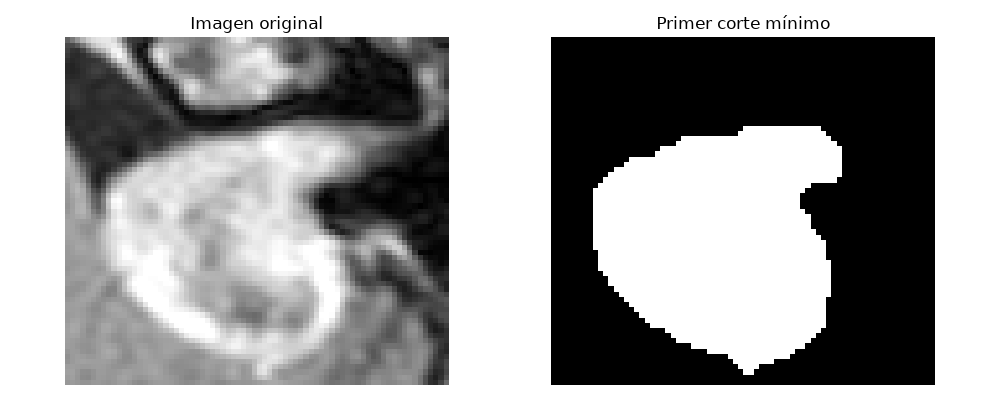
\includegraphics[width=0.95\textwidth]{vs-seg-001-primer-corte.png}
 \caption{Imagen de entrada y primer corte mínimo para
 \texttt{VS-SEG-001}, recortados al rectángulo seleccionado. El blanco
 representa el primer plano y el negro, el fondo en la segmentación.
 La región obtenida contiene 1685 píxeles. Figura exportada de la salida
 conservada en el cuaderno~\cite{cuaderno}; imagen de origen
 \cite{shapeydatos}.}
 \label{fig:primer-corte}
\end{figure}

\subsection{Evolución de la segmentación}

La primera iteración cambió 3273 etiquetas respecto de la inicialización,
en la que todos los píxeles interiores pertenecían al primer plano. La
segunda modificó 54 etiquetas y produjo una región de 1653 píxeles. Desde
la tercera hasta la quinta iteración no se registraron cambios en las
etiquetas. La tabla~\ref{tab:iteraciones} presenta las energías reducidas
antes y después de cada corte, calculadas con los modelos de esa iteración.

\begin{table}[!htbp]
 \centering
 \caption{Evolución de las cinco iteraciones para \texttt{VS-SEG-001}.
 Las energías corresponden a la ecuación~\eqref{eq:energia-reducida}.
 Cada comparación anterior--posterior utiliza los mismos parámetros
 gaussianos. Los valores se muestran con tres decimales.}
 \label{tab:iteraciones}
 \begin{tabular}{rrrr}
 \toprule
 Iteración & Etiquetas modificadas & Energía anterior & Energía posterior \\
 \midrule
 1 & 3273 & $33040{,}453$ & $29246{,}318$ \\
 2 & 54   & $28085{,}150$ & $28039{,}382$ \\
 3 & 0    & $28021{,}789$ & $28021{,}789$ \\
 4 & 0    & $28013{,}209$ & $28013{,}209$ \\
 5 & 0    & $27996{,}347$ & $27996{,}347$ \\
 \bottomrule
 \end{tabular}
\end{table}

La energía disminuyó durante los dos primeros cortes y permaneció igual
antes y después de los tres siguientes, a la precisión registrada.
Aunque las etiquetas no cambiaron en esas últimas iteraciones, la energía
varió entre ellas debido a la actualización de los modelos de intensidad.
La estabilidad observada corresponde a las etiquetas durante las cinco
iteraciones ejecutadas; no constituye una prueba de convergencia conjunta
de todos los parámetros.

\subsection{Comparación con la referencia}

La segmentación final presentó 47 falsos positivos y 84 falsos negativos,
para un total de 131 discrepancias. A partir de estos conteos y de los
1690 píxeles de referencia, se obtienen 1606 verdaderos positivos y 1653
píxeles clasificados como primer plano. La tabla~\ref{tab:evaluacion-caso}
compara el resultado con la predicción que asigna fondo a toda la imagen.

\begin{table}[!htbp]
 \centering
 \caption{Evaluación del caso \texttt{VS-SEG-001}. Los falsos positivos
 (FP) y falsos negativos (FN) se cuentan sobre la imagen completa.
 El error cuadrático medio (ECM) se calcula sobre 262\,144 píxeles para
 la imagen y sobre 4958 píxeles para el rectángulo.}
 \label{tab:evaluacion-caso}
 \begin{tabular}{lrrrr}
 \toprule
 Método & FP & FN & ECM global & ECM en el rectángulo \\
 \midrule
 GrabCut & 47 & 84 & $0{,}000500$ & $0{,}026422$ \\
 Todo fondo & 0 & 1690 & $0{,}006447$ & $0{,}340863$ \\
 \bottomrule
 \end{tabular}
\end{table}

El error de GrabCut equivale aproximadamente al $0{,}050$~\% de la
imagen y al $2{,}642$~\% del rectángulo. Frente a la predicción de todo
fondo, el número de discrepancias se redujo aproximadamente un
$92{,}25$~\%. Esta reducción se calcula con los conteos enteros, antes del
redondeo de las métricas. La referencia ocupa solo el $0{,}645$~\% de la
imagen, lo que explica que la predicción de todo fondo también presente
un error global pequeño pese a omitir completamente la lesión.

La figura~\ref{fig:evaluacion-final} muestra la anotación, la referencia,
la segmentación final y la distribución espacial de las discrepancias.
Los falsos positivos se observan principalmente en los extremos derecho
e inferior de la región, mientras que los falsos negativos aparecen en
porciones de su borde izquierdo e inferior. Predominan los píxeles de
lesión correctamente identificados en el interior. Las diferencias se
concentran en el límite de la región y no quedan descritas únicamente por
su área total.

\begin{figure}[!htbp]
 \centering
 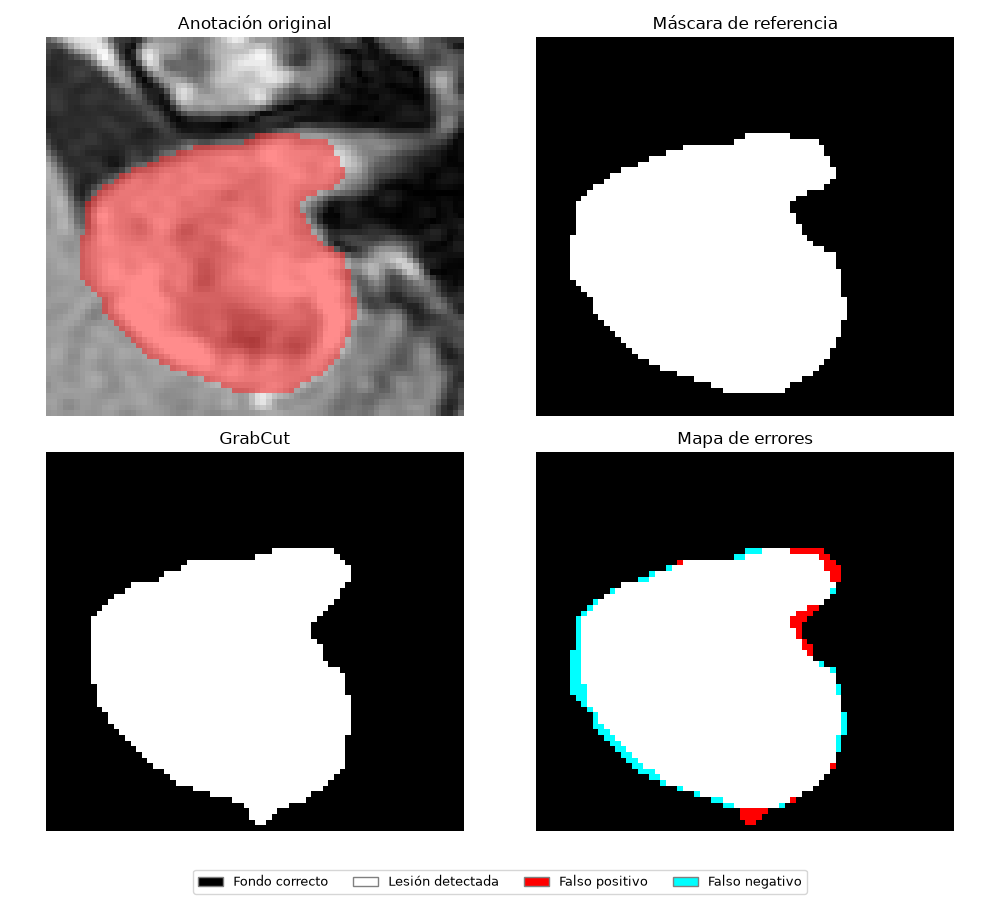
\includegraphics[width=0.86\textwidth]{vs-seg-001-evaluacion.png}
 \caption{Comparación final para \texttt{VS-SEG-001} dentro del rectángulo.
 Arriba: anotación roja y máscara binaria de referencia. Abajo:
 segmentación tras cinco iteraciones y mapa de errores. En este último,
 el blanco indica lesión correctamente identificada; el negro, fondo
 correcto; el rojo, falsos positivos; y el cian, falsos negativos.
 No hay píxeles de referencia fuera del rectángulo.
 Figura exportada de la salida conservada en el cuaderno~\cite{cuaderno}; imagen de origen
 \cite{shapeydatos}.}
 \label{fig:evaluacion-final}
\end{figure}

En el caso evaluado, la segmentación conservó la mayor parte de la región
anotada y las discrepancias se concentraron en sus bordes. Las etiquetas
se estabilizaron durante la ejecución, mientras continuaba el ajuste de
los modelos de intensidad.


% Descomenta cuando exista report/figures/resultado.png:
%
% \begin{figure}[htbp]
%   \centering
%   \includegraphics[width=0.85\textwidth]{resultado.png}
%   \caption{Resultado de la segmentación con GrabCut.}
%   \label{fig:resultado}
% \end{figure}

\FloatBarrier
% !TeX root = main.tex
\section{Conclusiones}
\label{sec:conclusiones}

La implementación de segmentación interactiva basada en GrabCut permitió
obtener una región compatible con la referencia disponible para el corte
\texttt{VS-SEG-001}, a partir de una inicialización rectangular. Tras cinco
iteraciones, se registraron 47 falsos positivos y 84 falsos negativos. El
error cuadrático medio fue de $0{,}000500$ sobre la imagen completa y de
$0{,}026422$ dentro del rectángulo. Frente a la predicción que asigna fondo
a todos los píxeles, las discrepancias se redujeron aproximadamente un
$92{,}25$~\% en este caso.

Las etiquetas permanecieron sin cambios desde la tercera iteración hasta
la quinta, aunque los modelos de intensidad continuaron actualizándose.
El procedimiento combina así el ajuste de los modelos de intensidad con
la minimización de la energía mediante cortes de grafos.

El predominio del fondo hace que el error global sea pequeño incluso
cuando se omite toda la lesión. Por ello, su interpretación requiere
considerar también el error dentro del rectángulo, los falsos positivos y
negativos y su distribución espacial. En el caso evaluado, las
discrepancias se concentraron en el límite de la región segmentada.

El caso estudiado ilustra la aplicación de GrabCut a la segmentación
interactiva de una lesión en resonancia magnética. La inicialización
rectangular delimita la región de búsqueda, los modelos gaussianos
describen las intensidades de ambas clases y los enlaces entre vecinos
favorecen la coherencia espacial de la región obtenida.


\clearpage
% !TeX root = main.tex
\begin{thebibliography}{11}
\addcontentsline{toc}{section}{Referencias}
\small

\bibitem{szeliski2011}
R. Szeliski (2011).
\textit{Computer Vision: Algorithms and Applications}.
Primera edición, Springer.
\href{https://doi.org/10.1007/978-1-84882-935-0}{doi:10.1007/978-1-84882-935-0}.

\bibitem{boykov2001}
Y. Y. Boykov y M.-P. Jolly (2001).
Interactive Graph Cuts for Optimal Boundary \& Region Segmentation
of Objects in N-D Images.
En \textit{Proceedings of the Eighth IEEE International Conference on Computer Vision}, vol.~1, pp.~105--112.
\href{https://doi.org/10.1109/ICCV.2001.937505}{doi:10.1109/ICCV.2001.937505}.

\bibitem{rother2004}
C. Rother, V. Kolmogorov y A. Blake (2004).
``GrabCut'': Interactive Foreground Extraction Using Iterated Graph Cuts. \textit{ACM Transactions on Graphics}, 23(3), 309--314.
\href{https://doi.org/10.1145/1015706.1015720}{doi:10.1145/1015706.1015720}.

\bibitem{shapeydatos}
J. Shapey, A. Kujawa, R. Dorent, G. Wang, S. Bisdas, A. Dimitriadis,
D. Grishchuck, I. Paddick, N. Kitchen, R. Bradford, S. Saeed, S. Ourselin
y T. Vercauteren (2021).
Segmentation of Vestibular Schwannoma from Magnetic Resonance Imaging:
An Open Annotated Dataset and Baseline Algorithm.
Versión~2, conjunto de datos \textit{Vestibular-Schwannoma-SEG},
The Cancer Imaging Archive, licencia CC BY 4.0.
\href{https://doi.org/10.7937/TCIA.9YTJ-5Q73}{doi:10.7937/TCIA.9YTJ-5Q73}.

\bibitem{clark2013}
K. Clark, B. Vendt, K. Smith, J. Freymann, J. Kirby, P. Koppel, S. Moore,
S. Phillips, D. Maffitt, M. Pringle, L. Tarbox y F. Prior (2013).
The Cancer Imaging Archive (TCIA): Maintaining and Operating a Public
Information Repository.
\textit{Journal of Digital Imaging}, 26(6), 1045--1057.
\href{https://doi.org/10.1007/s10278-013-9622-7}{doi:10.1007/s10278-013-9622-7}.

\bibitem{shapey2021}
J. Shapey, A. Kujawa, R. Dorent, G. Wang, A. Dimitriadis, D. Grishchuk,
I. Paddick, N. Kitchen, R. Bradford, S. R. Saeed, S. Bisdas, S. Ourselin
y T. Vercauteren (2021).
Segmentation of vestibular schwannoma from MRI, an open annotated
dataset and baseline algorithm.
\textit{Scientific Data}, 8, artículo~286.
\href{https://doi.org/10.1038/s41597-021-01064-w}{doi:10.1038/s41597-021-01064-w}.

\bibitem{presentacion}
F. Castro Chaves y E. Chacón Araya (2026).
\textit{Segmentación interactiva de tejidos con GrabCut: schwannoma
vestibular en resonancia magnética}.
Presentación del Foro Tema~4, PF-5039 Análisis de Imágenes, IIS-2026,
diapositivas~10--12 y~16. Material del proyecto no publicado.

\bibitem{cuaderno}
Proyecto \textit{horus-grabcut} (2026).
Cuaderno de segmentación interactiva \path{notebooks/grabcut.ipynb}
y archivos de \path{data/}.
Copia local consultada el 10 de octubre de 2026; se utilizan sus salidas
guardadas para \texttt{VS-SEG-001}. La copia local del cuaderno contiene
modificaciones respecto de la versión registrada en Git.
\href{https://github.com/DarthFranco2001/horus-grabcut}{Repositorio del proyecto}.

\bibitem{dinic1970}
E. A. Dinic (1970).
Algorithm for Solution of a Problem of Maximum Flow in Networks
with Power Estimation. \textit{Soviet Mathematics Doklady}, 11, 1277--1280.
\href{https://www.cs.bgu.ac.il/~dinitz/D70.pdf}{Texto de la publicación en el sitio del autor}.

\bibitem{repositorio}
Proyecto \textit{horus-grabcut} (2026).
\textit{horus-grabcut}. Repositorio de código fuente: cuaderno,
aplicación web, datos de trabajo y pruebas.
\url{https://github.com/DarthFranco2001/horus-grabcut}.

\bibitem{web}
Proyecto \textit{horus-grabcut} (2026).
\textit{Laboratorio GrabCut}. Aplicación web interactiva.
Consultada el 10 de octubre de 2026.
\url{https://darthfranco2001.github.io/horus-grabcut/}.

\end{thebibliography}


\end{document}